\section{Results}
\label{sec:results}

%% Auto-generated by tools/paper/generate_paper_assets.py
% Auto-generated paragraph – do not edit by hand.
The Digital Twin policy achieves a median handover latency of 13.40\,ms (P95: 19.94\,ms) with a success rate of 95.0\%. The Distance-Based policy achieves a median handover latency of 13.86\,ms (P95: 18.80\,ms) with a success rate of 100.0\%. The RL-Optimized policy achieves a median handover latency of 13.31\,ms (P95: 18.28\,ms) with a success rate of 96.2\%. The RSRP-Based policy achieves a median handover latency of 14.41\,ms (P95: 19.09\,ms) with a success rate of 100.0\%. Across all MEC services, the mean CPU utilisation is 61.5\% and the mean service latency is 2.78\,ms. The DQN agent converges at episode 23 with a final reward of 0.9340. The digital-twin achieves a KPI prediction accuracy of 94.3\% over 1200 predictions.


\subsection{Handover Performance}
Table~\ref{tab:handover_kpi} compares the three handover policies across
the pedestrian and vehicular scenarios.

%% Auto-generated by tools/paper/generate_paper_assets.py
\begin{table}[htbp]
  \centering
  \caption{Handover KPI Comparison (mean over all events)}
  \label{tab:handover_kpi}
  \begin{tabular}{@{}lccc@{}}
    \toprule
    \textbf{Algorithm} & \textbf{Success Rate} &
    \textbf{Latency (ms)} & \textbf{Tput Loss (ms)} \\
    \midrule
    Digital Twin & 95.0\% & 13.71 & -- \\
    Distance-Based & 100.0\% & 14.20 & -- \\
    RL-Optimized & 96.2\% & 14.78 & -- \\
    RSRP-Based & 100.0\% & 14.33 & -- \\
    \bottomrule
  \end{tabular}
\end{table}


Fig.~\ref{fig:latency_cdf} shows the CDF of handover latency for all three
algorithms in the pedestrian scenario.

\begin{figure}[htbp]
  \centering
  %% Auto-generated by tools/paper/generate_paper_assets.py
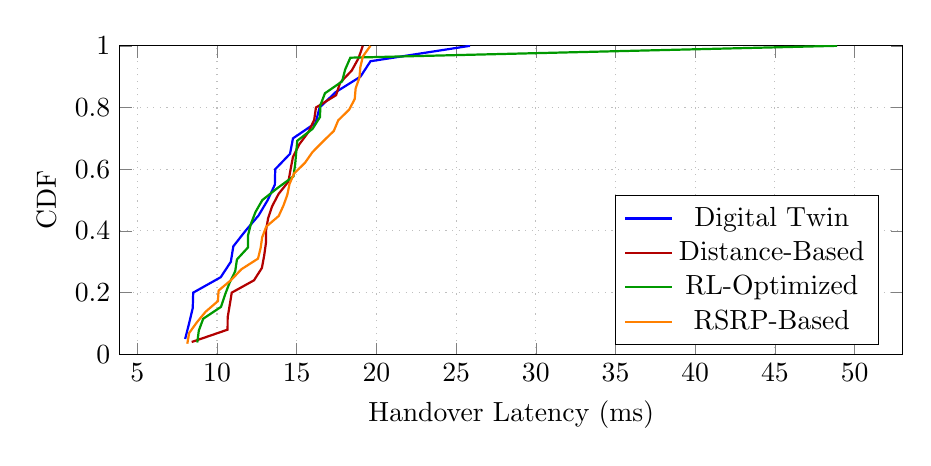
\begin{tikzpicture}
\begin{axis}[
  width=0.95\columnwidth, height=5.5cm,
  xlabel={Handover Latency (ms)},
  ylabel={CDF},
  ymin=0, ymax=1,
  legend pos=south east,
  grid=major, grid style={dotted},
  cycle list name=color list,
]
  \addplot[blue, thick] coordinates {(8.002,0.0500) (8.247,0.1000) (8.478,0.1500) (8.507,0.2000) (10.233,0.2500) (10.868,0.3000) (11.023,0.3500) (11.782,0.4000) (12.606,0.4500) (13.181,0.5000) (13.629,0.5500) (13.653,0.6000) (14.581,0.6500) (14.765,0.7000) (16.187,0.7500) (16.435,0.8000) (17.448,0.8500) (18.999,0.9000) (19.629,0.9500) (25.871,1.0000)};
  \addlegendentry{Digital Twin}
  \addplot[red!70!black, thick] coordinates {(8.412,0.0400) (10.664,0.0800) (10.668,0.1200) (10.799,0.1600) (10.925,0.2000) (12.321,0.2400) (12.816,0.2800) (12.959,0.3200) (13.067,0.3600) (13.069,0.4000) (13.202,0.4400) (13.459,0.4800) (13.863,0.5200) (14.480,0.5600) (14.617,0.6000) (14.766,0.6400) (15.153,0.6800) (15.729,0.7200) (16.098,0.7600) (16.207,0.8000) (17.470,0.8400) (17.719,0.8800) (18.454,0.9200) (18.881,0.9600) (19.146,1.0000)};
  \addlegendentry{Distance-Based}
  \addplot[green!60!black, thick] coordinates {(8.763,0.0385) (8.858,0.0769) (9.134,0.1154) (10.251,0.1538) (10.496,0.1923) (10.780,0.2308) (11.141,0.2692) (11.252,0.3077) (11.938,0.3462) (11.942,0.3846) (12.129,0.4231) (12.416,0.4615) (12.843,0.5000) (13.782,0.5385) (14.797,0.5769) (14.903,0.6154) (14.967,0.6538) (15.036,0.6923) (15.995,0.7308) (16.461,0.7692) (16.485,0.8077) (16.773,0.8462) (17.848,0.8846) (18.039,0.9231) (18.365,0.9615) (48.908,1.0000)};
  \addlegendentry{RL-Optimized}
  \addplot[orange, thick] coordinates {(8.138,0.0345) (8.252,0.0690) (8.731,0.1034) (9.281,0.1379) (10.054,0.1724) (10.102,0.2069) (10.897,0.2414) (11.533,0.2759) (12.573,0.3103) (12.736,0.3448) (12.834,0.3793) (13.087,0.4138) (13.869,0.4483) (14.173,0.4828) (14.411,0.5172) (14.546,0.5517) (14.834,0.5862) (15.517,0.6207) (15.984,0.6552) (16.643,0.6897) (17.328,0.7241) (17.606,0.7586) (18.291,0.7931) (18.641,0.8276) (18.697,0.8621) (18.934,0.8966) (18.993,0.9310) (19.150,0.9655) (19.625,1.0000)};
  \addlegendentry{RSRP-Based}
\end{axis}
\end{tikzpicture}

  \caption{CDF of handover latency for Distance-Based, RSRP-Based, and
           RL-Optimised policies (pedestrian scenario).}
  \label{fig:latency_cdf}
\end{figure}

\subsection{Throughput vs.\ Offered Load}
Fig.~\ref{fig:throughput_load} illustrates how aggregate throughput
scales with the number of active UEs under the three policies.

\begin{figure}[htbp]
  \centering
  %% Auto-generated by tools/paper/generate_paper_assets.py
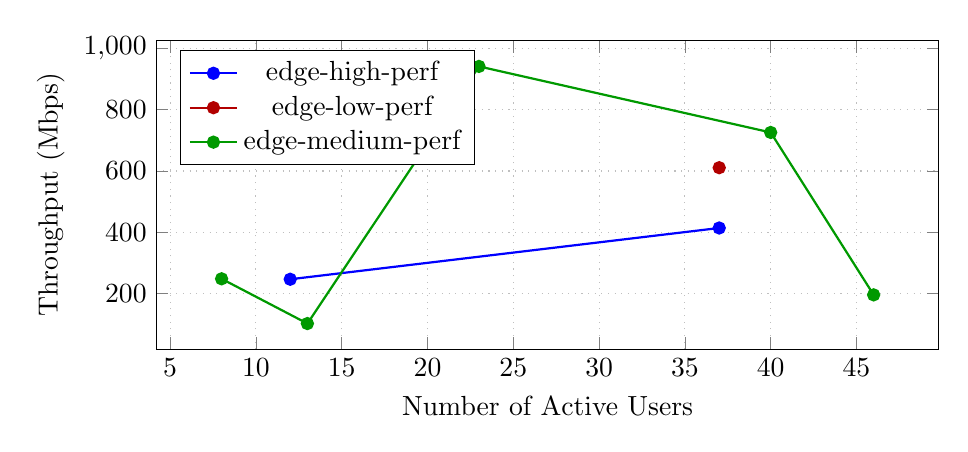
\begin{tikzpicture}
\begin{axis}[
  width=0.95\columnwidth, height=5.5cm,
  xlabel={Number of Active Users},
  ylabel={Throughput (Mbps)},
  legend pos=north west,
  grid=major, grid style={dotted},
]
  \addplot[blue, thick, mark=*] coordinates {(12.0,246.28) (37.0,413.72)};
  \addlegendentry{edge-high-perf}
  \addplot[red!70!black, thick, mark=*] coordinates {(37.0,610.66)};
  \addlegendentry{edge-low-perf}
  \addplot[green!60!black, thick, mark=*] coordinates {(8.0,247.77) (13.0,101.57) (23.0,941.46) (40.0,725.78) (46.0,195.25)};
  \addlegendentry{edge-medium-perf}
\end{axis}
\end{tikzpicture}

  \caption{Aggregate throughput vs.\ number of active UEs.}
  \label{fig:throughput_load}
\end{figure}

\subsection{RSRP/SINR Time Series}
Fig.~\ref{fig:rsrp_timeseries} shows representative RSRP and SINR
trajectories for a single UE during a handover event.

\begin{figure}[htbp]
  \centering
  %% Auto-generated by tools/paper/generate_paper_assets.py
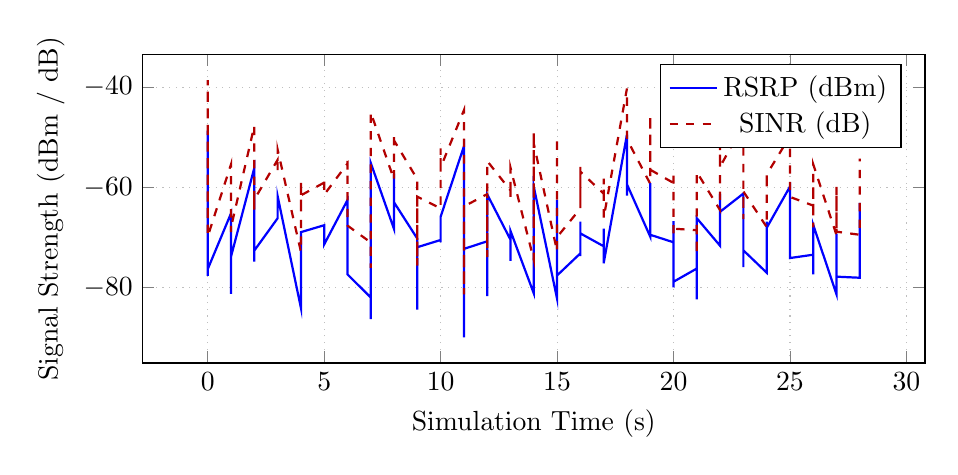
\begin{tikzpicture}
\begin{axis}[
  width=0.95\columnwidth, height=5.5cm,
  xlabel={Simulation Time (s)},
  ylabel={Signal Strength (dBm / dB)},
  legend pos=north east,
  grid=major, grid style={dotted},
]
  \addplot[blue, thick] coordinates {(0.00,-77.69) (0.00,-57.68) (0.00,-48.69) (0.00,-76.35) (1.00,-65.20) (1.00,-81.31) (1.00,-73.84) (2.00,-56.12) (2.00,-74.88) (2.00,-73.61) (2.00,-72.65) (3.00,-66.20) (3.00,-64.98) (3.00,-61.77) (4.00,-84.11) (4.00,-70.58) (4.00,-74.24) (4.00,-68.97) (5.00,-67.59) (5.00,-69.20) (5.00,-71.42) (6.00,-62.56) (6.00,-66.19) (6.00,-64.98) (6.00,-77.42) (7.00,-82.03) (7.00,-86.35) (7.00,-55.15) (8.00,-68.37) (8.00,-59.94) (8.00,-57.26) (8.00,-63.02) (9.00,-70.28) (9.00,-84.45) (9.00,-71.98) (10.00,-70.54) (10.00,-71.01) (10.00,-66.13) (10.00,-65.88) (11.00,-51.80) (11.00,-89.99) (11.00,-72.32) (12.00,-70.80) (12.00,-81.74) (12.00,-74.00) (12.00,-61.43) (13.00,-70.49) (13.00,-74.69) (13.00,-68.73) (14.00,-81.22) (14.00,-60.68) (14.00,-76.79) (14.00,-59.88) (15.00,-82.30) (15.00,-62.51) (15.00,-77.63) (16.00,-73.21) (16.00,-66.85) (16.00,-73.79) (16.00,-69.22) (17.00,-71.79) (17.00,-68.25) (17.00,-75.20) (18.00,-49.50) (18.00,-55.36) (18.00,-61.69) (18.00,-59.40) (19.00,-69.87) (19.00,-59.16) (19.00,-69.50) (20.00,-71.00) (20.00,-66.78) (20.00,-80.00) (20.00,-78.89) (21.00,-76.24) (21.00,-82.41) (21.00,-66.19) (22.00,-71.70) (22.00,-64.20) (22.00,-61.33) (22.00,-64.90) (23.00,-61.26) (23.00,-75.95) (23.00,-72.61) (24.00,-77.07) (24.00,-66.88) (24.00,-67.61) (24.00,-68.12) (25.00,-59.87) (25.00,-68.52) (25.00,-74.15) (26.00,-73.48) (26.00,-70.10) (26.00,-77.39) (26.00,-67.53) (27.00,-81.41) (27.00,-69.25) (27.00,-77.87) (28.00,-78.09) (28.00,-63.10)};
  \addlegendentry{RSRP (dBm)}
  \addplot[red!70!black, thick, dashed] coordinates {(0.00,-66.17) (0.00,-49.32) (0.00,-38.60) (0.00,-69.83) (1.00,-55.39) (1.00,-68.95) (1.00,-68.01) (2.00,-47.70) (2.00,-64.48) (2.00,-60.74) (2.00,-62.46) (3.00,-54.51) (3.00,-56.56) (3.00,-52.47) (4.00,-72.89) (4.00,-58.67) (4.00,-65.26) (4.00,-61.62) (5.00,-59.07) (5.00,-58.20) (5.00,-61.48) (6.00,-55.26) (6.00,-56.64) (6.00,-54.74) (6.00,-67.66) (7.00,-71.04) (7.00,-76.11) (7.00,-45.04) (8.00,-58.50) (8.00,-51.17) (8.00,-49.26) (8.00,-50.64) (9.00,-58.42) (9.00,-75.66) (9.00,-61.88) (10.00,-64.24) (10.00,-61.87) (10.00,-52.21) (10.00,-56.06) (11.00,-44.60) (11.00,-81.39) (11.00,-63.83) (12.00,-61.37) (12.00,-73.99) (12.00,-64.41) (12.00,-54.76) (13.00,-60.64) (13.00,-62.10) (13.00,-56.10) (14.00,-74.50) (14.00,-48.72) (14.00,-67.28) (14.00,-51.29) (15.00,-72.81) (15.00,-50.02) (15.00,-69.96) (16.00,-64.25) (16.00,-55.94) (16.00,-62.79) (16.00,-56.88) (17.00,-61.28) (17.00,-58.29) (17.00,-66.17) (18.00,-40.27) (18.00,-48.54) (18.00,-49.61) (18.00,-50.40) (19.00,-59.30) (19.00,-45.56) (19.00,-56.49) (20.00,-59.14) (20.00,-57.70) (20.00,-69.32) (20.00,-68.28) (21.00,-68.59) (21.00,-73.47) (21.00,-56.96) (22.00,-64.59) (22.00,-55.40) (22.00,-49.71) (22.00,-55.89) (23.00,-47.47) (23.00,-66.37) (23.00,-60.84) (24.00,-67.95) (24.00,-58.79) (24.00,-60.18) (24.00,-57.45) (25.00,-49.80) (25.00,-59.89) (25.00,-61.93) (26.00,-63.67) (26.00,-59.39) (26.00,-68.01) (26.00,-55.42) (27.00,-69.58) (27.00,-59.94) (27.00,-68.88) (28.00,-69.50) (28.00,-54.26)};
  \addlegendentry{SINR (dB)}
\end{axis}
\end{tikzpicture}

  \caption{RSRP and SINR time series for UE~0 illustrating a handover
           event (pedestrian scenario).}
  \label{fig:rsrp_timeseries}
\end{figure}

\subsection{MEC Service Performance}
Table~\ref{tab:mec_kpi} summarises MEC service utilisation and latency.

%% Auto-generated by tools/paper/generate_paper_assets.py
\begin{table}[htbp]
  \centering
  \caption{MEC Service KPI Summary}
  \label{tab:mec_kpi}
  \begin{tabular}{@{}lcccc@{}}
    \toprule
    \textbf{Service} & \textbf{Edge Node} &
    \textbf{CPU} & \textbf{Memory} & \textbf{Latency (ms)} \\
    \midrule
    Video Analytics & edge-high-perf & 48.3\% & 73.8\% & 4.79 \\
    IoT Data Processing & edge-medium-perf & 74.2\% & 54.6\% & 2.55 \\
    AR/VR Streaming & edge-high-perf & 82.8\% & 75.8\% & 1.95 \\
    Federated Learning & edge-medium-perf & 57.6\% & 42.0\% & 4.67 \\
    Video Analytics & edge-medium-perf & 34.2\% & 47.9\% & 1.04 \\
    IoT Data Processing & edge-medium-perf & 63.2\% & 75.4\% & 3.17 \\
    AR/VR Streaming & edge-low-perf & 80.9\% & 72.8\% & 1.58 \\
    Federated Learning & edge-medium-perf & 51.2\% & 61.1\% & 2.51 \\
    \bottomrule
  \end{tabular}
\end{table}


\subsection{Federated Learning Convergence}
The FL xApp converged after the episode reported in
Table~\ref{tab:ml_summary} with the final reward and prediction accuracy
summarised therein.

%% Auto-generated by tools/paper/generate_paper_assets.py
\begin{table}[htbp]
  \centering
  \caption{AI/ML Module Summary}
  \label{tab:ml_summary}
  \begin{tabular}{@{}lcc@{}}
    \toprule
    \textbf{Module} & \textbf{Metric} & \textbf{Value} \\
    \midrule
    RL (DQN) & Final reward & 0.9340 \\
    RL (DQN) & Convergence episode & 23 \\
    Digital Twin & Prediction accuracy & 94.3\% \\
    Digital Twin & Total predictions & 1200 \\
    Digital Twin & Correct predictions & 1132 \\
    \bottomrule
  \end{tabular}
\end{table}

